\documentclass{article}
\usepackage[utf8]{inputenc}

\usepackage[paperwidth=8.5in, paperheight=11in, top=1in, bottom=.5in, left=.5in, right=.5in]{geometry}
\usepackage{fancyhdr, graphicx,tikz,amsmath,multicol,paracol,pgfplots}
\usepackage[inline]{enumitem}


\pagestyle{fancy}
\lhead{\large{\textbf{Module 5: Exponential and Logarithmic Functions - Readiness Assurance Test}}}
\chead{}
\rhead{}
\lfoot{}
\cfoot{}
%\rfoot{\thepage/\pageref{LastPage} }
\setlength{\headheight}{14pt} %added in bc warning

%%% LIST ANSWER KEY HERE

% 1 C
% 2 B
% 3 C
% 4 D
% 5 A
% 6 D
% 7 A
% 8 D
% 9 C
% 10 B


\begin{document}


\begin{enumerate}


% % WRITE WHICH READINESS OBJECTIVE THE PROBLEM GOES WITH AS COMMENT

% \item Sample question with 4 answers in one column. (Tag correct answer with comment.)

%   \begin{enumerate}
  
%   \item first answer choice  %correct 
%   \item second answer choice
%   \item third answer choice
%   \item fourth answer choice
  
%   \end{enumerate}

% % objective description

% \item Sample question with four answers on one row. 

%   \begin{enumerate}
%   \begin{multicols}{4}
%   \item first answer choice  %correct 
%   \item second answer choice
%   \item third answer choice
%   \item fourth answer choice
%   \end{multicols}
%   \end{enumerate}

% Simplify expressions using properties of exponents.

\item Which expression is equivalent to $x^2\cdot x^3$?

  \begin{enumerate}
  \begin{multicols}{4}
      \item $x^{-1}$ 
      \item $x^{1}$ 
      \item $x^{5}$  %correct
      \item $x^{6}$ 
  \end{multicols}
  \end{enumerate}  


\item Which expression is equivalent to $\dfrac{x^8}{x^2}$?

  \begin{enumerate}
  \begin{multicols}{4}
      \item $x^{10}$  
      \item $x^{6}$ %correct
      \item $x^{16}$  
      \item $x^{-6}$ 
  \end{multicols}
  \end{enumerate}  


\item Which expression is equivalent to $(x^3)^{5}$?

  \begin{enumerate}
  \begin{multicols}{4}
      \item $x^{8}$  
      \item $x^{-2}$ 
      \item $x^{15}$  %correct
      \item $x^{2}$ 
  \end{multicols}
  \end{enumerate}  



% Simplify expressions that involve negative exponents.

\item Which expression is equivalent to $\dfrac{1}{2x^5}$?

  \begin{enumerate}
  \begin{multicols}{4}
      \item $2x^{5}$  
      \item $2x^{-5}$ 
      \item $\dfrac{1}{2}x^{5}$  
      \item $\dfrac{1}{2}x^{-5}$ %correct
  \end{multicols}
  \end{enumerate}  


% Graph functions using transformations.

\item If $f(x)$ is the function graphed below, which graph represents $-f(x+1)-3$?
        \begin{center}
        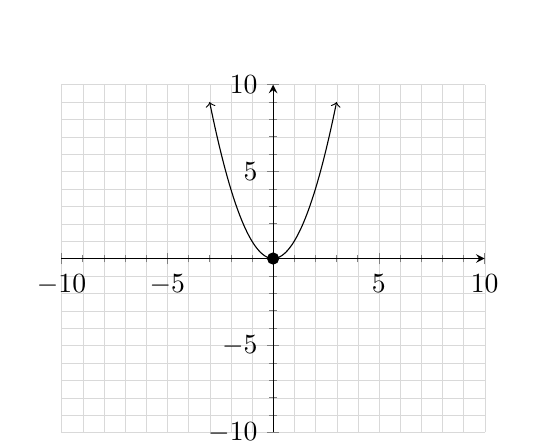
\begin{tikzpicture}
        \begin{axis}[
                height=6cm,
                axis lines=center,
                grid=both,
                grid style={line width=.05pt, draw=gray!30},
                minor tick num=4,
                xtick={-10,-5,...,10},
                ytick={-10,-5,...,10},
                xmin=-10, xmax=10,
                ymin=-10, ymax=10,
                ]
                \addplot [
                    domain=-3:3, 
                    samples=200, 
                    color=black,
                    <->,
                    ]{x^2};
                \addplot[mark=*] coordinates {(0,0)};
        \end{axis}
        \end{tikzpicture}
        \end{center}

  \begin{enumerate}
  \begin{multicols}{2}
        \item 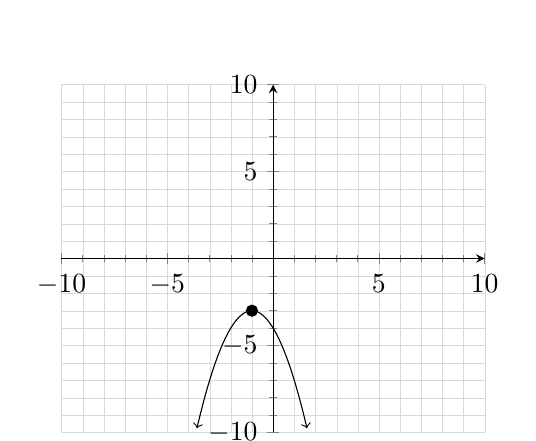
\begin{tikzpicture}   %correct
        \begin{axis}[
                height=6cm,
                axis lines=center,
                grid=both,
                grid style={line width=.05pt, draw=gray!30},
                minor tick num=4,
                xtick={-10,-5,...,10},
                ytick={-10,-5,...,10},
                xmin=-10, xmax=10,
                ymin=-10, ymax=10,
                ]
                \addplot [
                    domain=-3.6:1.6, 
                    samples=200, 
                    color=black,
                    <->,
                    ]{-(x+1)^2-3};
                \addplot[mark=*] coordinates {(-1,-3)};
        \end{axis}
        \end{tikzpicture}

        \item 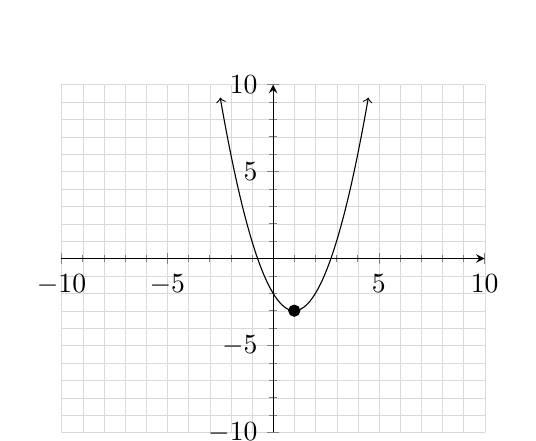
\begin{tikzpicture}
        \begin{axis}[
                height=6cm,
                axis lines=center,
                grid=both,
                grid style={line width=.05pt, draw=gray!30},
                minor tick num=4,
                xtick={-10,-5,...,10},
                ytick={-10,-5,...,10},
                xmin=-10, xmax=10,
                ymin=-10, ymax=10,
                ]
                \addplot [
                    domain=-2.5:4.5, 
                    samples=200, 
                    color=black,
                    <->,
                    ]{(x-1)^2-3};
                \addplot[mark=*] coordinates {(1,-3)};
        \end{axis}
        \end{tikzpicture}

        \item 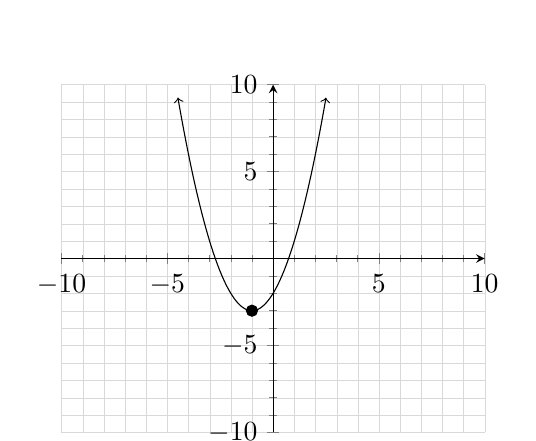
\begin{tikzpicture}   
        \begin{axis}[
                height=6cm,
                axis lines=center,
                grid=both,
                grid style={line width=.05pt, draw=gray!30},
                minor tick num=4,
                xtick={-10,-5,...,10},
                ytick={-10,-5,...,10},
                xmin=-10, xmax=10,
                ymin=-10, ymax=10,
                ]
                \addplot [
                    domain=-4.5:2.5, 
                    samples=200, 
                    color=black,
                    <->,
                    ]{(x+1)^2-3};
                \addplot[mark=*] coordinates {(-1,-3)};
        \end{axis}
        \end{tikzpicture}

        \item 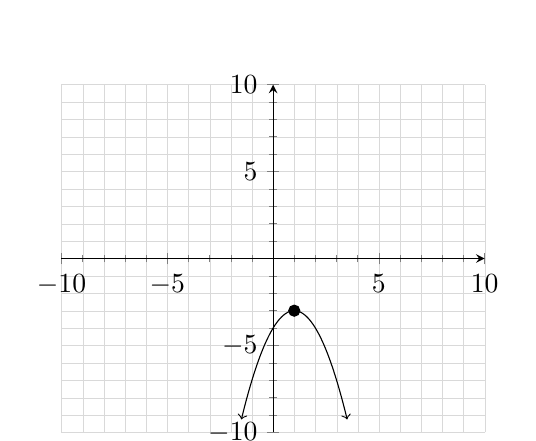
\begin{tikzpicture}   
        \begin{axis}[
                height=6cm,
                axis lines=center,
                grid=both,
                grid style={line width=.05pt, draw=gray!30},
                minor tick num=4,
                xtick={-10,-5,...,10},
                ytick={-10,-5,...,10},
                xmin=-10, xmax=10,
                ymin=-10, ymax=10,
                ]
                \addplot [
                    domain=-1.5:3.5, 
                    samples=200, 
                    color=black,
                    <->,
                    ]{-(x-1)^2-3};
                \addplot[mark=*] coordinates {(1,-3)};
        \end{axis}
        \end{tikzpicture}
    
      
  \end{multicols}
  
  \end{enumerate}


% Solve linear inequalities.

\item Solve the linear inequality given below. Express your answer in interval notation.

\[ 7-2x \geq 13 \] 

  \begin{enumerate}
  \begin{multicols}{4}
      \item $(-3, \infty)$ 
      \item $(-\infty, -3)$ 
      \item $[-3, \infty)$  
      \item $(-\infty, -3]$  %correct
  \end{multicols}
  \end{enumerate}  

% Find the domain and range of a function from its graph.
\vspace{5pt}
\hspace{-15pt}\textbf{The function $f(x)$ is pictured below. Use this graph for questions 7-8.}

        \begin{center}
        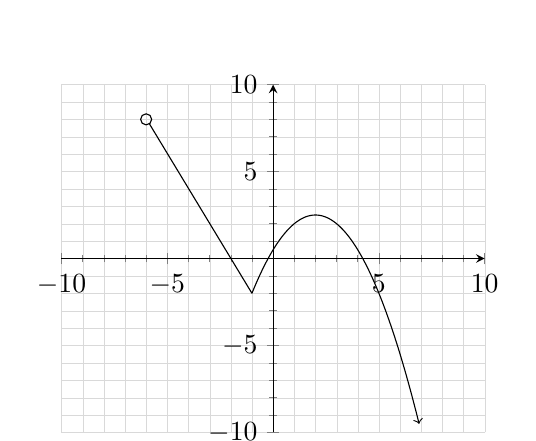
\begin{tikzpicture}   
        \begin{axis}[
                height=6cm,
                axis lines=center,
                grid=both,
                grid style={line width=.05pt, draw=gray!30},
                minor tick num=4,
                xtick={-10,-5,...,10},
                ytick={-10,-5,...,10},
                xmin=-10, xmax=10,
                ymin=-10, ymax=10,
                ]
                \addplot [mark= ] coordinates {(-5.85,7.75) (-1,-2)};
                %\addplot [mark=* ] coordinates {(-1,-2)};
                \addplot [mark=o ] coordinates {(-6,8)};
                \addplot [
                    domain=-1:6.9, 
                    samples=200, 
                    color=black,
                    ->,
                    ]{-0.5*(x-2)^2+2.5};
                
        \end{axis}
        \end{tikzpicture}              
        \end{center}

\item Find the domain of $f(x)$.        

        \begin{enumerate}
        \begin{multicols}{4}
              \item $(-6, \infty)$ %correct 
              \item $(-\infty, 8)$
              \item $(-6, 7)$
              \item $(-10,10)$ 
        \end{multicols}
        \end{enumerate}  

\item Find the range of $f(x)$.      

        \begin{enumerate}
        \begin{multicols}{4}
              \item $(-9.5, 8)$, 
              \item $(-10,10)$ 
              \item $(-6, \infty)$ 
              \item $(-\infty, 8)$ %correct 
              
        \end{multicols}
        \end{enumerate}  

% Determine horizontal and vertical asymptotes from a graph.

\vspace{5pt}
\hspace{-15pt}\textbf{The function $g(x)$ is pictured below. Use this graph for questions 9-10.}

        \begin{center}
        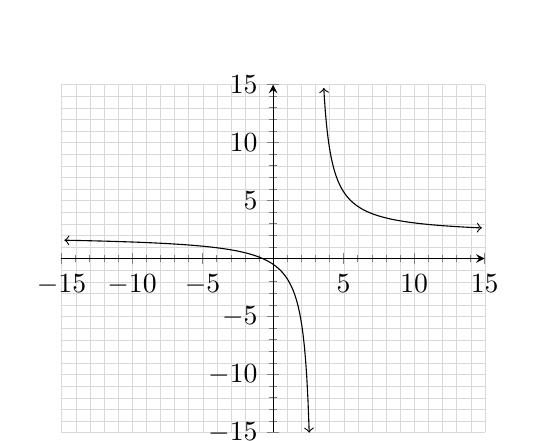
\begin{tikzpicture}   
        \begin{axis}[
                height=6cm,
                axis lines=center,
                grid=both,
                grid style={line width=.05pt, draw=gray!30},
                minor tick num=4,
                xtick={-15,-10,...,15},
                ytick={-15,-10,...,15},
                xmin=-15, xmax=15,
                ymin=-15, ymax=15,
                ]
                \addplot [
                    domain=-14.8:2.56, 
                    samples=200, 
                    color=black,
                    <->,
                    ]{(4*x+3)/(2*x-6)};
                \addplot [
                    domain=3.59:14.8, 
                    samples=200, 
                    color=black,
                    <->,
                    ]{(4*x+3)/(2*x-6)};
                
        \end{axis}
        \end{tikzpicture}              
        \end{center}

\item Find the equation of the horizontal asymptote of $g(x)$.


        \begin{enumerate}
        \begin{multicols}{4}
              \item $x=2$
              \item $x=3$
              \item $y=2$ %correct
              \item $y=3$
        \end{multicols}
        \end{enumerate} 


\item Find the equation of the vertical asymptote of $g(x)$.

        \begin{enumerate}
        \begin{multicols}{4}
              \item $x=2$
              \item $x=3$ %correct
              \item $y=2$ 
              \item $y=3$
        \end{multicols}
        \end{enumerate}  


 
  

\end{enumerate}


\end{document}